\documentclass{article}
\usepackage{template/iclr2026_conference,times}
\usepackage[T1]{fontenc}
\usepackage[utf8]{inputenc}
\usepackage{microtype,graphicx,booktabs,amsmath,amssymb,array,tabularx,multirow,seqsplit}
\usepackage[dvipsnames,table]{xcolor}
\usepackage{caption,float}
\usepackage{url}
\usepackage[colorlinks=true,linkcolor=MidnightBlue,citecolor=MidnightBlue,urlcolor=MidnightBlue]{hyperref}
\iclrfinalcopy
\urlstyle{same}
\definecolor{paperblue}{HTML}{245C91}
\captionsetup{font=small,labelfont=bf,skip=10pt,justification=raggedright,singlelinecheck=false}
\captionsetup[figure]{skip=10pt}
\definecolor{tablewash}{HTML}{EEF4F9}
\renewcommand{\arraystretch}{1.15}
\newcolumntype{Y}{>{\raggedright\arraybackslash}X}
\setlength{\textfloatsep}{12pt}
\setlength{\intextsep}{10pt}
\setlength{\tabcolsep}{5pt}
\setlength{\abovedisplayskip}{10pt plus 2pt minus 2pt}
\setlength{\belowdisplayskip}{10pt plus 2pt minus 2pt}
\setlength{\abovedisplayshortskip}{10pt plus 2pt minus 2pt}
\setlength{\belowdisplayshortskip}{10pt plus 2pt minus 2pt}
\raggedbottom
\newcommand{\pct}{\%}
\newcommand{\code}[1]{\texttt{\small #1}}
\newcommand{\Hbeta}{H_{\beta}}
\title{\normalfont\LARGE\bfseries Knolling Bot: Language-Guided Object Arrangement}
\author{Minjae Bang\\
Department of Computer Science\\
Columbia University
\And
Hod Lipson\\
Department of Mechanical Engineering\\
Columbia University}
\hypersetup{pdftitle={Knolling Bot: Language-Guided Object Arrangement},pdfauthor={Minjae Bang, Hod Lipson},pdfsubject={Language-conditioned object arrangement; course research paper}}
\begin{document}
\maketitle
\vspace{-8pt}
\lhead{}
\rhead{}
\renewcommand{\headrulewidth}{0pt}
\begin{abstract}
We present a system that predicts object arrangements from overhead RGB images and English instructions. It combines object-centric perception, learned row and order prediction, and geometric placement to satisfy constraints on selection, orientation, grouping, and spacing. On an independent set of 128 scene families and 640 image--instruction pairs, our system achieves 540/640 strict successes (84.4\%), compared with 489/640 (76.4\%) for its predecessor using the same learned base. It preserves every previous success and gains 8.0 percentage points (95\% family-bootstrap interval 4.8--11.6). The results support a staged hybrid approach to instruction-conditioned arrangement and identify spacing as the main remaining source of failure in this synthetic setting.
\end{abstract}
\vspace{-8pt}
\begin{figure}[H]
\centering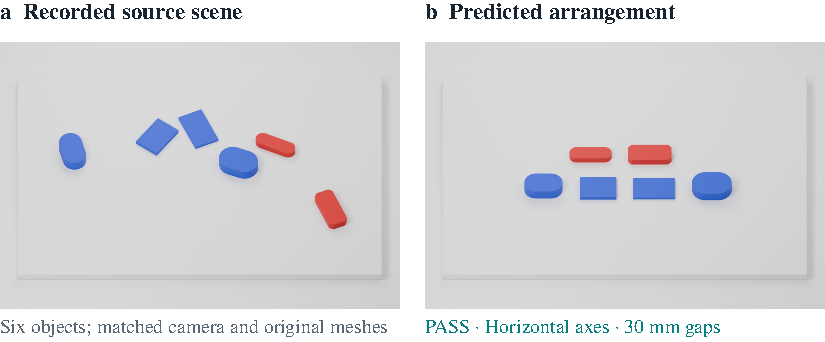
\includegraphics[width=0.84\linewidth]{figures/qualitative_full_annotated.pdf}
\caption{\textbf{Language-guided arrangement.} Matched Blender views show a saved six-object validation prediction with the original meshes and poses. The instruction requests horizontal axes, increasing area, and 30\,mm gaps. The prediction uses the original overhead RGB input.}
\label{fig:qualitative}
\end{figure}
\vspace{-10pt}
\section{Introduction}
Knolling organizes objects into aligned, evenly spaced layouts for assembly preparation. A visually tidy arrangement can still move an unselected object, violate a gap, or extend beyond the requested region. Satisfying a complete instruction requires perception, language grounding, and geometric reasoning to work together.

We study full-arrangement, color-selective, and no-op commands for two to eight objects. The system predicts discrete layout structure (row membership and object order) before placing objects according to estimated dimensions and requested gaps. Held objects retain their estimated source poses, with no teacher poses used at inference. A paired evaluation on independent scene families measures improvement, while failure analysis identifies the constraints that still limit complete-scene success.

\paragraph{Related work.}
Knolling Bot predicts tidy placements sequentially \citep{hu2025knolling}, and \emph{Knolling Bot 2.0} estimates graspability for clutter \citep{hu2023knolling2}. These published Columbia systems are separate from the project reported here. StructFormer uses point clouds for language-guided structure \citep{liu2022structformer}, whereas Transporter Networks and CLIPort predict manipulation actions \citep{zeng2021transporter,shridhar2022cliport}. We evaluate complete geometric validity from calibrated RGB and language. Task differences preclude direct performance comparisons.

\clearpage
\section{Method}
\label{sec:method}
Given overhead RGB $I\in[0,1]^{3\times384\times576}$ and an English instruction $t$, the system predicts planar poses $\hat P=\{(\hat x_i,\hat y_i,\hat\theta_i)\}_{i=1}^{\hat N}$ in a $0.60\times0.40$\,m workspace. Orientation follows the undirected long axis and is therefore $\pi$-periodic. Commands arrange all objects, select a color, or preserve the scene. Preferences specify the region, 15/20/30\,mm gaps, color grouping, area order, and orientation. A vertical-orientation command rotates objects while rows continue to run left to right.

\vspace{2pt}
\begin{figure}[H]
\centering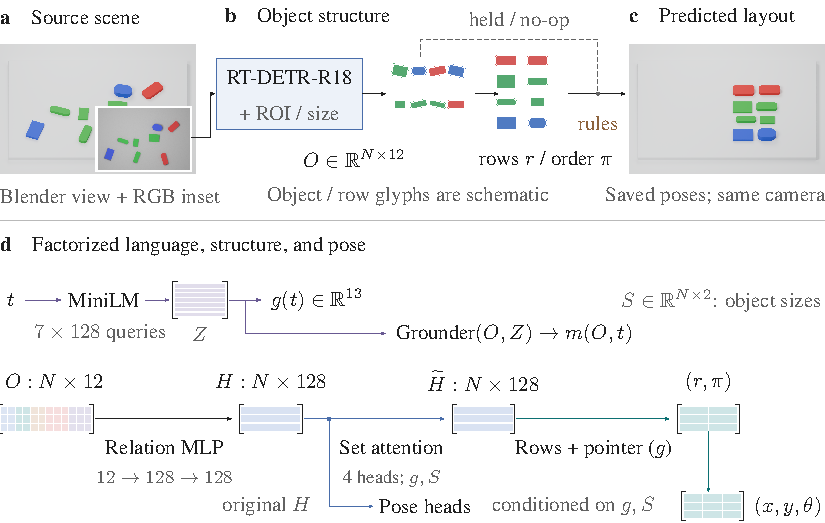
\includegraphics[width=\linewidth]{figures/architecture_main.pdf}
\caption{\textbf{Hybrid inference and learned layout.} The RGB inset shows the model input, and the rendered views depict stored poses. Tensor symbols denote schemas for variable $N$. Seven attention slots $Z$ support the text-only goal $g$ and object-conditioned selection $m$. Contextual features predict $(r,\pi)$, while pose heads use the original $H$. Geometry refines movers while held and no-op objects retain estimated source poses.}
\label{fig:architecture}
\end{figure}
\vspace{-10pt}

\paragraph{Perception and language grounding.}
RT-DETR-R18 \citep{zhao2024rtdetr}, a DETR-based detector \citep{carion2020detr}, produces object queries and physical attributes. Crop-conditioned appearance and size heads refine each detection into a 12-dimensional representation of position, size, angle, color, and shape. MiniLM \citep{wang2020minilm,reimers2020multilingual} encodes the instruction, and seven learned queries pool its tokens into a 13-dimensional global goal. A separate object--language attention branch identifies the objects to move. Template rules correct predicted region or gap categories that conflict with explicit English commands.

\paragraph{Learned structure and constrained coordinates.}
A relation encoder produces features $h_i\in\mathbb R^{128}$. Four-head set attention conditions row assignment $r$ and pointer order $\pi$ on the goal and object sizes, while the pose heads use the original $h_i$. The initial search ranks structures by row and order log-probabilities and checks at most eight candidates. Full arrangements also enforce predicted-area order. For feasible aligned neighbors, placement satisfies
\begin{equation}\label{eq:mainspacing}
 \hat x_{j+1}-\hat x_j=\tfrac12(\hat w_j+\hat w_{j+1})+d,\qquad |d-\delta|\leq2\,\mathrm{mm},
\end{equation}
where $\hat w_j$ is the rotated horizontal extent and $\delta$ is the requested gap. Row heights similarly determine vertical spacing. This separates the choice of structure from placement using estimated dimensions. Conditional repair ranks alternative rows by their probabilities and retains the original prediction if its bounded search fails. The procedure does not guarantee a feasible layout.

\paragraph{Selective preservation.}
For partial arrangements, the system selects the named color and searches for translations around objects that must remain in place. Held and no-op objects retain detected centers. Their angles are estimated from RGB silhouettes by principal-component analysis, with a learned fallback. Preservation thus depends on the accuracy of the source-pose estimates. Appendix~\ref{app:implementation} gives the routing and search bounds.

\section{Data, Training, and Evaluation}
\label{sec:protocol}
\paragraph{Synthetic corpus.}
The corpus contains 4,000 geometry families and 20,000 image--instruction pairs. Each RGB image is paired with three full-arrangement commands, one color-selective command, and one no-op command, allowing the instruction to vary while the scene remains fixed. Procedural boxes, chamfers, and capsules appear in red, green, or blue. A geometric teacher generates target layouts, an independent validator checks them, and Blender Cycles renders the images. The train/validation/test split contains 3,200/400/400 families, corresponding to 16,000/2,000/2,000 pairs. This separation keeps identical source images out of different splits. Individual training stages use the subsets described below.

\paragraph{Staged optimization.}
Perception and arrangement models are first trained separately. Relation stages then use 791 training pairs and 94 validation pairs, followed by a size-residual stage supervised on source dimensions. Restricted joint fine-tuning updates the size residual and selected row-coordinate parameters while freezing perception, language, goal, relation, row assignment, order, and angle heads. Refined sizes are detached before pose computation, so pose loss cannot train perception. The selector learns row and pointer assignments from 5,085 usable full-arrangement pairs among 5,376 eligible pairs from 1,792 training families. Detection-count or association checks exclude 291 pairs. Eight epochs are recorded, and epoch 1 is selected on 1,200 full validation pairs. Appendix~\ref{app:training} details the losses, hyperparameters, gradient boundaries, and development diagnostics.

A broader joint-training pilot was not adopted because performance deteriorated. By update 200, success had fallen from 2/38 to 0/38 on development and from 24/152 to 1/152 on validation. The final system therefore retains the staged approach. This outcome concerns one configuration and leaves effective system-wide joint optimization an open research question.

\paragraph{Sealed release comparison.}
The final evaluation uses a later, separately generated set of 128 families and 640 pairs. Its family IDs, RGB hashes, and asset-family IDs are disjoint from the 20,000-pair corpus. Objects come from the development asset pool not rendered in that corpus, while retaining the same procedural shapes and colors. The set contains 384 full, 127 partial, and 129 no-op pairs. Both releases use the same records, evaluator, and thresholds. Neither this set nor the official 2,000-pair test split was used to select checkpoints or thresholds. We analyze the stored sealed scores without rerunning inference or selecting another model.

\paragraph{Strict complete-scene success.}
A prediction fails immediately if the object count is wrong. Otherwise, Hungarian matching associates predicted source objects with true identities, subject to a 10\,mm center-error limit and envelope IoU $\geq0.5$. The evaluator then checks target poses using true object geometry. Success requires every applicable check to pass, including selection and preservation, region, axis, row alignment, gaps, color grouping, size order, collision, clearance, and boundary constraints. The score averages these binary scene outcomes,
\begin{equation}
 S=\frac{1}{M}\sum_{s=1}^{M}\mathbf{1}\{\hat N_s=N_s\ \land\ \text{identity and task checks pass}\}.
\end{equation}
A valid arrangement can pass even if it differs from the teacher layout. The metric evaluates instruction fulfillment at the pose level rather than visual aesthetics, grasp success, trajectory safety, or physical execution.

\begin{table}[H]
\centering\small
\caption{Prediction-scoring thresholds. Dataset acceptance is checked separately and requires stored locked poses to copy the source exactly.}
\label{tab:tolerances}
\begin{tabular*}{\linewidth}{@{}l@{\extracolsep{\fill}}l@{}}\toprule
\textbf{Check} & \textbf{Threshold / requirement} \\\midrule
Held position / long-axis angle & $\leq1$\,mm / $\leq1^\circ$ deviation \\
Requested axis / row alignment & $\leq2^\circ$ / $\leq2$\,mm deviation \\
Horizontal / vertical gap & $\leq2$\,mm from requested gap \\
Object clearance / table margin & At least 10\,mm (0.1\,mm numerical tolerance) \\
Size order & At most 5\% area inversion \\\bottomrule
\end{tabular*}
\end{table}

\section{Results and Analysis}
\label{sec:results}
\paragraph{Paired release comparison.}
v1.0.0 is the baseline implementation, and v2.0.0 keeps that learned model while refining inference; these releases are not published \emph{Knolling Bot 2.0} \citep{hu2023knolling2}. Table~\ref{tab:main} evaluates one bundle: 10\,mm duplicate suppression, sentence-consistent region and gap choices, stricter named-color selection, and feasibility-gated row and color repair.

\begin{table}[H]
\centering
\caption{Strict target-layout success on the independent 640-pair set. Each count gives successful scenes over evaluated scenes, and gains are paired differences in percentage points.}
\label{tab:main}
\begin{tabularx}{\linewidth}{Yrrr}\toprule
\textbf{Task} & \textbf{v1.0.0} & \textbf{v2.0.0} & \textbf{Gain (pp)} \\\midrule
Full & 287/384 (74.7\%) & 311/384 (81.0\%) & +6.3 \\
Partial & 84/127 (66.1\%) & 104/127 (81.9\%) & +15.7 \\
No-op & 118/129 (91.5\%) & 125/129 (96.9\%) & +5.4 \\\midrule
\rowcolor{tablewash} Overall & 489/640 (76.4\%) & \textbf{540/640 (84.4\%)} & \textbf{+8.0} \\\bottomrule
\end{tabularx}
\end{table}

v2.0.0 retains all 489 v1.0.0 successes and adds 51, comprising 24 full, 20 partial, and 7 no-op scenes. Failures fall from 151 to 100, a 33.8\% relative reduction. Because five instructions share each image, we bootstrap paired \emph{families} rather than individual commands. Across 10,000 resamples, the 95\% interval is +4.8 to +11.6 percentage points. Twenty-nine families improve, 99 tie, and none worsen. This interval describes variation across evaluation families for the frozen systems, not training-seed uncertainty or real-world domain shift.

\begin{figure}[H]
\centering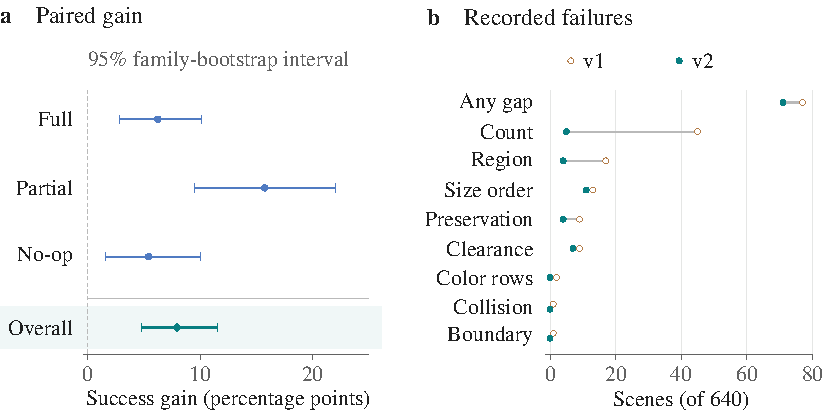
\includegraphics[width=0.96\linewidth]{figures/holdout_diagnostics.pdf}
\caption{\textbf{Release-level gains and remaining errors.} (a) Paired success gains with pointwise 95\% family-bootstrap intervals. (b) Recorded error counts for the two releases. ``Any gap'' combines horizontal and vertical violations. Tags can overlap, and count failures skip subsequent checks.}
\label{fig:results}
\end{figure}

\paragraph{Patterns of improvement and failure.}
Partial tasks show the largest gain. Count failures decrease from 45 to 5 and region failures from 17 to 4, consistent with the intended refinements. Eight-object success rises from 47/90 to 65/90 (52.2\% to 72.2\%), although it remains below the two-object result of 91/95 for both releases. Without component ablations, these changes cannot be attributed to individual rules.

Spacing remains the dominant source of failure. The 49 horizontal-gap and 42 vertical-gap failures overlap in 20 scenes, so 71/100 failed scenes violate at least one gap constraint. Other tags include 11 size-order, 7 clearance, 5 count, 4 region, and 4 preservation errors. One possible explanation is that placement uses \emph{predicted} dimensions whereas scoring uses true bounding rectangles. A layout can pass its internal feasibility check yet miss the scored gap threshold. The tags do not establish how often this mechanism occurs.

\section{Interpreting Predicted Arrangements}
\label{sec:discussion}
\begin{figure}[H]
\centering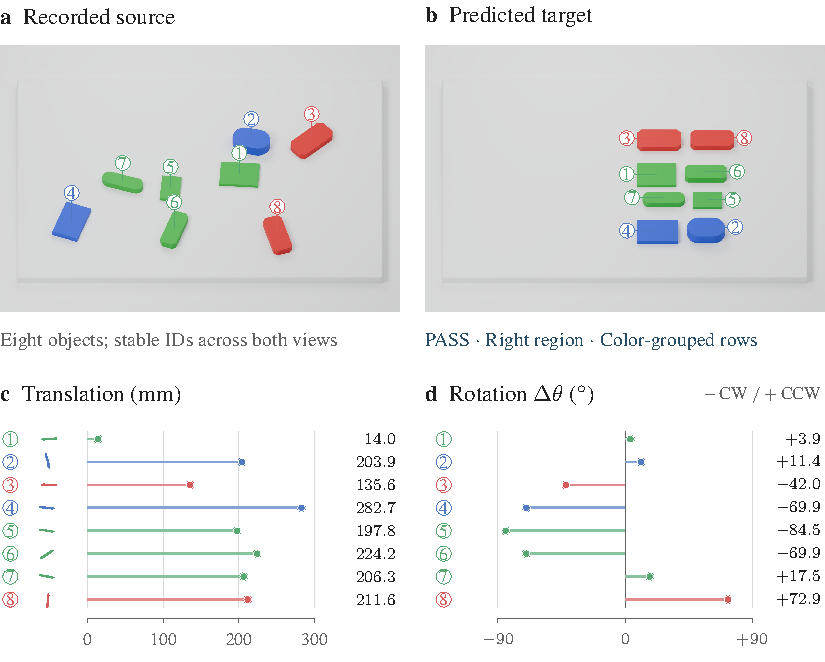
\includegraphics[width=\linewidth]{figures/motion_correspondence.pdf}
\caption{\textbf{Object-wise predicted motion.} IDs link recorded source poses to predicted targets. In (c), equal-length arrows show direction ($+x$ right, $+y$ up), while dots and labels show displacement. In (d), $\Delta\theta\in[-90^\circ,90^\circ)$ is the counterclockwise-positive change modulo $180^\circ$. These endpoint differences do not specify robot trajectories. Appendix~\ref{app:motionaudit} gives the coordinates and spacing analysis.}
\label{fig:motion}
\end{figure}

\paragraph{From pose changes to task validity.}
Figure~\ref{fig:motion} shows a modest change for object 1 (14.0\,mm, $+3.9^\circ$) and a larger displacement for object 4 (282.7\,mm, $-69.9^\circ$), both within a valid final layout. Figures~\ref{fig:modes}--\ref{fig:diagnostics} illustrate the limits of judging such layouts visually. A full-layout row gap exceeds its upper limit by 0.657\,mm. In the partial layout, the closest footprints are 12.820\,mm apart, yet their envelopes miss the effective 9.9\,mm clearance limit by 3.9\,$\mu$m. The visibly separated pair fails because of conservative scoring geometry, not a visible collision. This numerical margin does not imply physical positioning precision.

\paragraph{Scope and limitations.}
The system achieves RGB-and-language inference through staged learning, discrete selection, template correction, image-based angle estimation, and geometric search. We have not yet demonstrated joint training across the full pipeline. Evaluation is limited to calibrated synthetic scenes with three colors and three shape types, containing at most eight objects. Real images, paraphrases, severe occlusions, and physical execution have not been tested. Using one learned base without factorial ablations or multiple seeds also limits component attribution and uncertainty estimation. Appendix~\ref{app:reproducibility} describes the available runtime and reproducibility evidence.

\section{Conclusion}
Our approach achieves 84.4\% strict scene success on an independent, family-separated set, improving on its predecessor by 8.0 percentage points. The results support combining learned layout structure with geometric placement and selective preservation. Future work should improve spacing, isolate the effects of individual refinements, and evaluate joint training and physical execution.

\begingroup
\small
\raggedright
\bibliography{references}
\bibliographystyle{template/iclr2026_conference}
\endgroup
\clearpage
\appendix
\section{Appendix}
\subsection{Implementation Details}
\label{app:implementation}
\paragraph{Coordinates and object representation.}
Positions are measured in meters from the workspace's bottom-left corner, and angles counterclockwise from $+x$ in radians, modulo $\pi$. Image coordinates follow $p_x=576x/0.6-0.5$, $p_y=384(1-y/0.4)-0.5$. Each object is represented by
\begin{equation}
 o_i=[x_i/0.6,\ y_i/0.4,\ a_i/0.6,\ b_i/0.4,\ \cos(2\theta_i),\ \sin(2\theta_i),\ c_i^{(1:3)},\ q_i^{(1:3)}],
\end{equation}
where $a_i,b_i$ are the predicted major and minor dimensions, and $c_i,q_i$ are color and shape probabilities. Inference accepts one to eight detections, while evaluated scenes contain two to eight objects.

\begin{table}[H]
\centering\small
\caption{Dimensions and operations in the adopted inference pipeline.}
\begin{tabularx}{\linewidth}{@{}lY@{}}\toprule
\textbf{Component} & \textbf{Implementation} \\\midrule
Perception & RT-DETR-R18; 3 decoder layers; 300 width-256 queries; internal $640\times640$ input. \\
Appearance adapter & $16\times16$ predicted-box crop; CNN $3\to16\to32$; query/crop head $288\to128\to10$. \\
Size residual & $8\times8$ crop; 16-channel CNN feature + query; MLP $272\to64\to2$; dimension floor $10^{-4}$\,m. \\
Language & MiniLM tokens $384\to128$; 7 goal queries; four-head text attention; feed-forward $128\to512\to128$. \\
Goal / selection & Text-only goal: keep (1), axis (2), region (3), gap (3), grouping (2), order (2). Separate selection: object $12\to128$, self-/language attention, head $128\to1$. \\
Relation / context & MLP $12\to128\to128$; one width-128, four-head set-attention block for structure. \\
Structure & Row MLP $141\to128\to8$; pointer query $269\to128\to128$, masked dot-product selection. \\
Pose heads & Row origin $417\to128\to2$; X step $3\to32\to1$; angle $141\to128\to2$, half-atan2 decoding. \\
Filtering / search & Foreground threshold 0.5; duplicate-center radius 10\,mm; at most eight checked candidates per search. \\\bottomrule
\end{tabularx}
\end{table}

For keep probability $k$ and attribute distributions $p_a,p_r,p_\delta,p_c,p_s$, the goal is $g=[k,(1-k)p_a,(1-k)p_r,(1-k)p_\delta,(1-k)p_c,(1-k)p_s]$. The set-context block normalizes tokens $z_i=h_i+W_g g+W_s s_i$ and adds its self-attention output to $h_i$. A null key handles padding. The contextual features guide row and order selection, while the pose heads use the original $h_i$. Rows and pointer prefixes are predicted at inference and teacher-forced during training. Objects in a row share their neural origin's $y$ coordinate, and positive X steps use $\operatorname{softplus}(\operatorname{MLP}([w_{j-1},w_j,\delta]))$.

The ideal axis-aligned spacing is
\begin{equation}
 x_{j+1}-x_j=\tfrac12(w_j+w_{j+1})+\delta,\qquad
 y_r-y_{r+1}=\tfrac12(H_r+H_{r+1})+\delta_r,
\label{eq:spacing}
\end{equation}
where $w_j$ is horizontal extent, $H_r$ is the maximum row height, and $\delta_r=2\delta$ between color bands ($\delta$ otherwise). The decoder uses rotated rectangles and accepts $\pm2$\,mm gap bands around these ideal equalities. The regions $(x_{\min},y_{\min},x_{\max},y_{\max})$ are full $(.02,.02,.58,.38)$, left $(.02,.02,.28,.38)$, and right $(.32,.02,.58,.38)$. A fitting layout may shift 1\,mm inward.

The initial search ranks candidates by row and pointer scores, whereas repair and color-split searches use row scores. Enumeration may consider additional partitions before truncation. Area order is explicitly enforced on the full route and during repair, but not throughout the partial route. If repair is exhausted, the original prediction is retained, so neither feasibility nor global optimality is guaranteed.

\paragraph{Preservation implementation.}
Partial mode replaces the mover set for an unambiguous named color, then searches block translations on a 5\,mm grid within $\pm120$\,mm around held objects. Held/no-op angles use silhouette PCA on connected components in a local $\pm80$\,mm window, with chroma threshold $25/255$ and at least 40 pixels. The fallback proceeds through the direction head to the detector angle. Centers come from detections. This yields static placements without trajectory planning.

\subsection{Training Evidence and Optimization}
\label{app:training}
\begin{table}[H]
\centering\small
\caption{Recorded training stages and data use. The counts describe each stage rather than repeated training on the full corpus. The official test set and independent final holdout are excluded.}
\begin{tabularx}{\linewidth}{@{}lY@{}}\toprule
\textbf{Stage} & \textbf{Evidence and scope} \\\midrule
Base integration & Separate perception and arrangement checkpoints at updates 2,400 and 6,000, respectively. \\
Relation stages & 791 training and 94 validation pairs; seed 1203. The final pipeline reuses only the relation hidden encoder. \\
Size residual & 3,200 train source families, divided into 2,560 fit / 640 development; batch 8; learning rate $10^{-3}$; selected update 200. \\
Restricted joint & Official train families split 4/5 fit, 1/5 development; batch 4; AdamW, learning rate $10^{-5}$, weight decay 0; 30 updates, 120 attempted presentations, 6 excluded. \\
Set selector & 1,792 eligible train families, 5,376 full pairs, 5,085 usable; 249 association and 42 count exclusions; 8 epochs / 1,272 updates; initial learning rate $10^{-4}$; selected epoch 1. \\
Broad joint pilot & Seed 1203; batch 2; encoder / goal / hidden / row learning rates $10^{-6}/10^{-5}/10^{-5}/10^{-4}$; stopped at update 200 after collapse; not adopted. \\\bottomrule
\end{tabularx}
\end{table}

\paragraph{Losses and gradient boundaries.}
Define the SmoothL1 penalty as $H_\beta(e)=e^2/(2\beta)$ for $|e|<\beta$ and $|e|-\beta/2$ otherwise, and let $d_\pi(\alpha,\beta)=((\alpha-\beta+\pi/2)\bmod\pi)-\pi/2$. The size residual minimizes
\begin{equation}
 \mathcal L_{\mathrm{size}}=\operatorname{mean}_{i\in M,k\in\{a,b\}}H_{.001}(\hat s_{ik}-s^*_{ik}).
\end{equation}
Here, $M$ denotes matched objects. Matching uses true source centers only during supervision, with detector outputs and predicted crop boxes detached. The selector's recorded objective combines row cross-entropy with teacher-forced pointer cross-entropy,
\begin{equation}
 \mathcal L_{\mathrm{select}}=\operatorname{CE}(R,r^*)+\operatorname{CE}(O,\pi^*),
\end{equation}
with invalid and padded targets ignored. These two losses account for the recorded total. The logs provide no evidence of an additional color regularizer.

In restricted joint fine-tuning, let $G$ contain reference predictions within 2\,mm position error and $3^\circ$ angle error, and $F$ contain the other valid objects. The recorded objective is
\begin{align}
\mathcal L_{\mathrm{joint}}={}&\mathcal L_{\mathrm{size}}
+\operatorname{mean}_{i\in F,k\in\{x,y\}}H_{.010}(\hat p_{ik}-p^*_{ik})
+\operatorname{mean}_{i\in F}|d_\pi(\hat\theta_i,\theta_i^*)|\nonumber\\
&+\operatorname{mean}_{i\in G,k\in\{x,y\}}H_{.001}(\hat p_{ik}-p^{\mathrm{ref}}_{ik}).
\end{align}
Empty terms contribute zero. Updates are restricted to the size residual, horizontal step head, and final row-origin layer. Refined sizes are detached before the pose forward pass, while perception, language, goal, relation, structure, and angle heads remain frozen. The angular term therefore contributes to the loss value without training the angle head. These gradient boundaries prevent joint optimization through the entire pipeline.

\paragraph{Development evidence and its limits.}
On the saved 152-scene full-arrangement diagnostic, success rises from 24 to 42 after size refinement and from 42 to 54 after restricted joint tuning. Size refinement reduces median major-dimension error from 1.419 to 0.790\,mm across 796 matched objects, while restricted joint tuning reduces median vertical-gap error from 2.015 to 1.588\,mm. Because code and selection gates changed across these development stages, the comparisons are not independent final-test ablations. The broader joint pilot instead falls from 2/38 to 0/38 development successes and from 24/152 to 1/152 validation successes at update 200, leaving update 0 as the best checkpoint. A historical 260-scene diagnostic overlapped earlier fitting data and is excluded from claims of independent generalization.

\subsubsection{Selector Learning Curve}
\begin{figure}[H]
\centering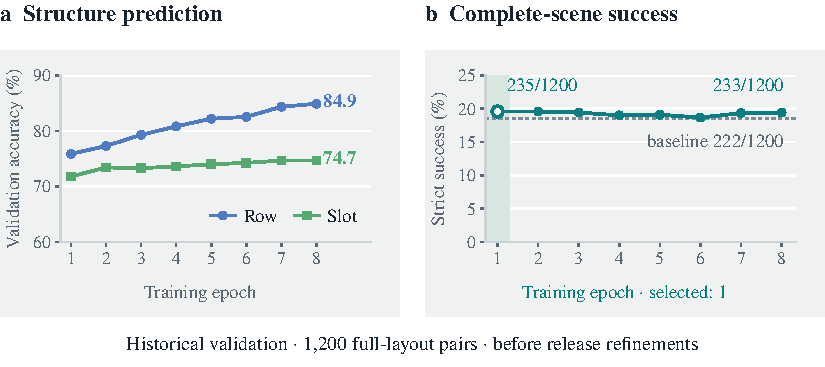
\includegraphics[width=\linewidth]{figures/selector_training.pdf}
\caption{Historical selector validation on 1,200 full-arrangement pairs. Row and slot accuracy improve while complete-scene success plateaus. The dashed line marks the recorded 222/1200 baseline, and shading identifies the selected epoch 1. This component-training diagnostic precedes the final inference refinements and independent evaluation.}
\label{fig:training}
\end{figure}

Epoch 1 improves success from the 222/1200 baseline to 235/1200. Row/slot accuracy rises to 75.86\%/71.77\% from 68.52\%/61.87\%, and mixed-color-row tags fall from 234 to 22. At epoch 8, accuracy reaches 84.88\%/74.68\%, but success is 233/1200. The later gains in row and slot accuracy did not improve complete-scene success.

\subsection{Data and Statistical Details}
\label{app:statistics}
Scene and asset seeds are 120912/120913. Major/minor dimensions span 40--80/25--50\,mm and heights 5--20\,mm on a 1\,mm grid, with aspect ratio $\geq1.3$. Teacher and instruction modes are \code{continuous\_rows\_v3}/\code{english\_rows\_v1}. For family $i$, bucket $\lfloor i/20\rfloor\bmod10$ assigns 0--7 to training, 8 to validation, and 9 to testing, with 64 disjoint asset families per split. Source clearance/margin is 12\,mm. Independently validated targets require 10\,mm and exact source copies for locked poses. Blender 5.1.0 renders RGB using Cycles CPU and 32 samples; PNG bytes may vary across environments.

The final set uses scene seed 20261112, registry seed 120913, and development assets. Its 128 families/640 pairs share no geometry-family IDs, RGB hashes, or asset-family IDs with the corpus. Teacher-derived mode labels classify already-satisfied selective commands as no-op. This labeling yields the 384 full, 127 partial, and 129 no-op cases used in the evaluation.

\paragraph{Paired bootstrap.}
Define $d_f=\frac15\sum_{j=1}^{5}(Y^{v2}_{fj}-Y^{v1}_{fj})$, with superscripts denoting v2.0.0 and v1.0.0. We resample 128 families with replacement and compute $100\operatorname{mean}_f d_f$, retaining paired commands. Python's local random generator (seed 20261112) produces 10,000 replicates. Sorted indices 250 and 9749 yield the interval [4.84375, 11.5625] points. Mode-specific intervals use the same draws and replicate-specific mode denominators. Paired counts are 489 both-pass, 51 v2.0.0-only, 0 v1.0.0-only, and 100 both-fail. This analysis reaggregates existing evaluations.

% The error table starts the next page. Ragged bottom keeps the shortfall
% at the foot of the page instead of stretching the section and paragraph skips.
\vfill
\begin{table}[H]
\centering\small
\caption{Error tags recorded for v1.0.0 or v2.0.0. Tags can overlap, including horizontal and vertical gap errors in 20 v2.0.0 scenes.}
\begin{tabular*}{\linewidth}{@{}l@{\extracolsep{\fill}}rrlrr@{}}\toprule
\textbf{Error} & \textbf{v1.0.0} & \textbf{v2.0.0} & \textbf{Error} & \textbf{v1.0.0} & \textbf{v2.0.0} \\\midrule
Horizontal gap & 51 & 49 & Clearance & 9 & 7 \\
Vertical gap & 48 & 42 & Keep pose & 9 & 4 \\
Object count & 45 & 5 & Mixed-color row & 2 & 0 \\
Requested region & 17 & 4 & Collision & 1 & 0 \\
Size order & 13 & 11 & Boundary & 1 & 0 \\\bottomrule
\end{tabular*}
\end{table}

\flushbottom
\subsection{Command Dependence and Object Correspondence}
\label{app:qualitative}
\begin{figure}[H]
\centering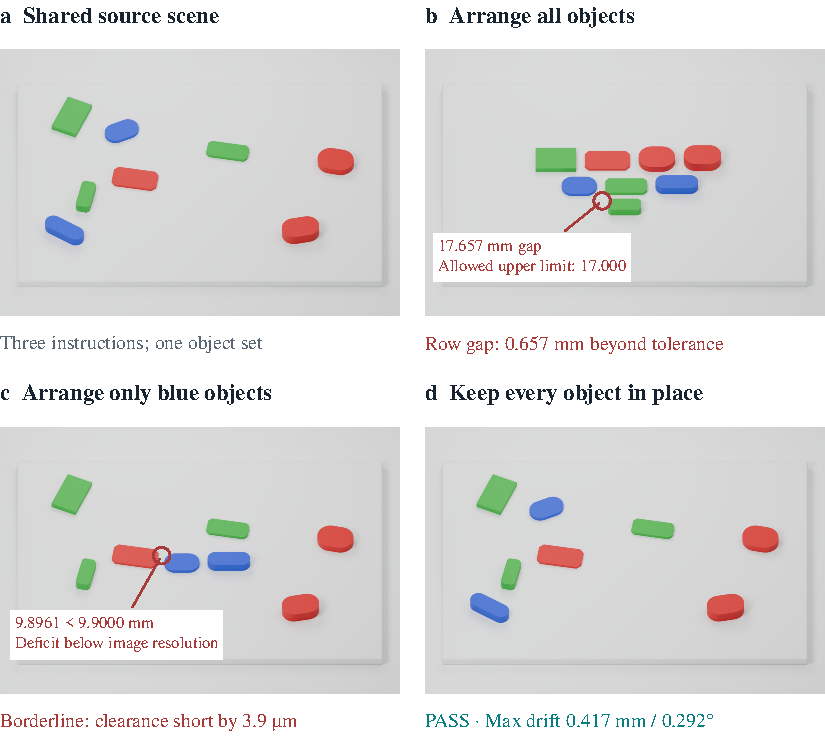
\includegraphics[width=\linewidth]{figures/qualitative_modes.pdf}
\caption{One validation scene under three commands, rendered with the same Blender camera and lighting. (b) fails because a row gap is 0.657\,mm past its upper limit. (c) fails clearance by 3.9\,$\mu$m, a deficit this print cannot resolve. (d) passes, with at most 0.42\,mm and 0.29$^\circ$ of drift from the source. Figure~\ref{fig:diagnostics} measures (b) and (c) on overhead crops.}
\label{fig:modes}
\end{figure}

\paragraph{Interpreting command-dependent layouts.}
The full and partial commands differ in which objects may move, while the no-op command requires the scene to remain unchanged. The two rejected arrangements show why visual plausibility alone is insufficient. Figure~\ref{fig:diagnostics} examines their scoring margins. Figure~\ref{fig:motion} provides a complementary view of object correspondence for an eight-object example, whose poses and geometry are detailed in Appendix~\ref{app:motionaudit}.

\paragraph{Example provenance.}
The smoke script selected the first supported example of each mode from family \code{expanded\_09aa3f57968449ce8a09f291}, with suffixes \code{\_0}, \code{\_2}, and \code{\_3}. The full and partial commands request horizontal axes and 15\,mm gaps, with partial mode selecting blue objects. Maximum no-op drift is 0.417\,mm and $0.292^\circ$. The six-object opening example is \code{expanded\_e2ee7a75ae3a34826b36d71f\_0}, and the eight-object motion example is \code{expanded\_717287879ce16878c5558650\_4}. These validation records illustrate behavior but lack per-record checkpoint digests and do not constitute a second benchmark. The older ten-image v1.0.0 gallery is excluded from the v2.0.0 evidence.

\subsection{Failure Margins and Rendering Fidelity}
\label{app:failure}
\begin{figure}[H]
\centering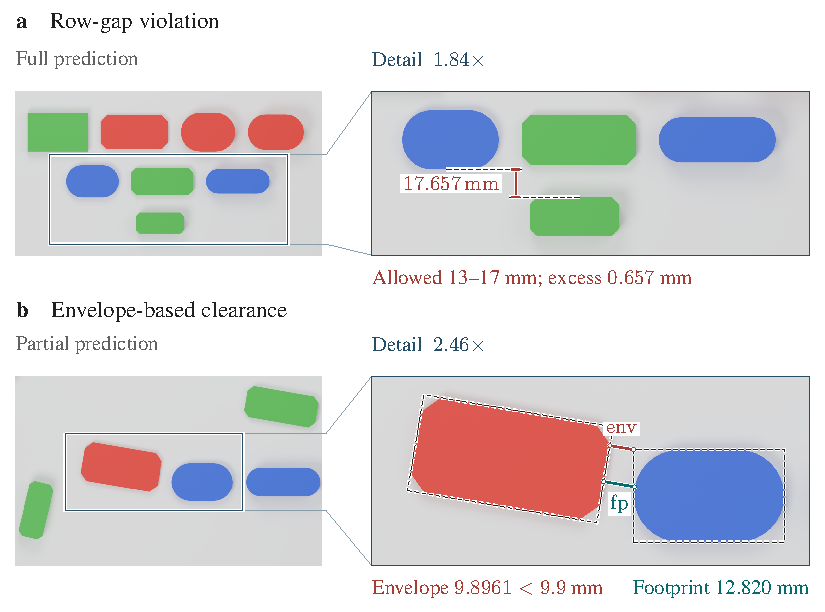
\includegraphics[width=\linewidth]{figures/failure_explanation.pdf}
\caption{\textbf{Why visual separation can still fail the geometric score.} Linked frames connect each saved prediction to a magnified view, where dashed outlines mark scored envelopes. The full layout exceeds its 13--17\,mm row-gap interval. In the partial layout, the closest footprints are 12.820\,mm apart, yet their envelopes are separated by 9.8961\,mm. This is 3.9\,$\mu$m below the effective 9.9\,mm minimum, a difference smaller than the render can resolve.}
\label{fig:diagnostics}
\end{figure}

\paragraph{Why the borderline example matters.}
The partial failure arises from conservative evaluation geometry rather than a visible collision. For objects o06/o08, the minimum distance between footprint polygons is 12.81985\,mm, while their oriented rectangular envelopes are 9.89610\,mm apart. Both distances are recomputed from saved poses, and this pair also has the smallest footprint separation in the complete scene. The 10\,mm clearance rule includes a 0.1\,mm numerical allowance. The example explains the recorded rejection, but cannot establish physical feasibility or how often this mechanism occurs across the holdout.

\paragraph{Pose and geometry fidelity.}
Every presentation image is rendered from a preserved scene record. Meshes extrude the original footprint polygons to their recorded heights, retaining object identity, color, dimensions, and source/predicted pose. Layouts are never adjusted for composition. Before/after views share the orthographic camera, illumination, materials, background, and image quality. Blender 5.1.0 uses Cycles CPU, denoising, and adaptive sampling with a 128-sample maximum. Overview images are $1920\times1280$, and dedicated closeups are $2040\times765$ and $2040\times885$. The closeups change only camera framing and resolution, preserving meshes, poses, materials, and lights.

The original $576\times384$ RGB images remain the inference inputs, as illustrated in Figure~\ref{fig:architecture}; presentation renders are generated afterward. The package includes input/output hashes, object transforms, camera settings, editable Blender scenes, and scripts. An independent check reopens each saved scene and compares every object transform and mesh vertex with the source record. Residual differences are limited to float32 storage quantization, below $10^{-7}$ in the corresponding meter/radian coordinates. This rendering and verification process performs no additional model inference or training.

\subsection{Reproducibility and Evidence Package}
\label{app:reproducibility}
The analysis compares v1.0.0 (\code{26dca53}) with v2.0.0 (\code{593bd5d}). These project releases are distinct from published \emph{Knolling Bot 2.0}. The comparison carries forward the release-candidate measurement without changing inference. Manuscript preparation used checkout \code{535f14f}. The adopted entry points are \code{load\_adopted} in the end-to-end scorer and \code{poses\_from\_detection} in \code{size\_refinement.py}. Source-identity matching minimizes a Hungarian cost based on confidence, source position, size, and angle. Every match must also satisfy center distance $\leq10$\,mm and oriented-envelope IoU $\geq0.5$. Otherwise, the scene fails with \code{source\_identity}. Matched target poses then undergo independent semantic and geometry checks.

The model runtime uses Python 3.12, PyTorch 2.9.1, torchvision 0.24.1, and transformers 4.57.3. Its text backbone is \code{paraphrase-multilingual-MiniLM-L12-v2}, with pretrained snapshots pinned in \code{configs/pretrained\_rtdetr.json}. Reloading requires local base/parent checkpoints, relation, joint row/size and selector weights, selection/direction heads, and pretrained caches. The repository distributes neither these weights nor the datasets, and the historical selector trainer and independent-set generator are missing. The package therefore reproduces the \emph{paper's analysis and figures}, but does not support full training reproduction.

\paragraph{Version-controlled change.}
The v1.0.0--v2.0.0 release changes refine inference through duplicate suppression, sentence-consistent region/gap choices, exact named-color mover replacement, infeasible-row repair, and feasible color-row splitting. Both versions share the architecture, loading paths, set attention, size residual, constraint search, and PCA correction. The effects of individual refinements have not been measured.

\begin{table}[H]
\centering\small
\caption{Contents of the manuscript evidence package. Paths are relative to the submission root; audit manifests preserve full SHA-256 values and original paths.}
\label{tab:package}
\begin{tabularx}{\linewidth}{@{}lY@{}}\toprule
\textbf{Artifact} & \textbf{Purpose} \\\midrule
\code{audit/evidence/v1\_holdout.jsonl} & Frozen baseline scores; SHA-256 prefix \code{89b3ee1cbc24}. \\
\code{audit/evidence/v2\_holdout.jsonl} & Frozen v2.0.0 scores; prefix \code{209df3c1b12c}. \\
\code{audit/verified\_results.json} & Recomputed counts, breakdowns, paired gain and family bootstrap. \\
\code{scripts/audit\_results.py} & Statistical reaggregation without model inference. \\
\code{scripts/make\_figures.py} & Figure rebuild entry point; calls the publication compositor. \\
\code{scripts/render\_publication.py} & Blender source for matched views at saved poses. \\
\code{renders/} & High-resolution PNGs, editable Blender scenes, and pose/camera metadata. \\
\code{audit/evidence/} & Training summaries, qualitative poses, RGB and rendered prediction. \\
\code{audit/method\_audit.md} & Claim-to-code references and gradient boundaries. \\
\code{audit/results\_audit.md} & Claim-to-record references and dataset integrity. \\
\code{template/upstream.json} & Official ICLR template source and exact hashes. \\\bottomrule
\end{tabularx}
\end{table}

\paragraph{Compute scope.}
The selector stage records 1,719 GPU-seconds, which covers only that stage. Saved inference timings give median 131.5/137.2\,ms and mean 169.2/197.5\,ms for v1.0.0/v2.0.0. Hardware, warmup, and serving conditions are insufficiently controlled for a throughput claim. The records do not establish total training compute, deployment cost, or a physical cycle time.

\paragraph{Rebuilding.}
The README provides commands and dependency pins, and the scripts in Table~\ref{tab:package} reconstruct the statistics and eight figures. The manuscript compiles with \code{latexmk -pdf main.tex}. Because all figure PDFs are included, compilation requires no Python environment, GPU, checkpoints, or original datasets.

\paragraph{Assistance disclosure.}
Codex assisted with repository and record inspection, primary-source literature discovery, drafting, figure scripting, and LaTeX typesetting. All experimental outcomes are drawn from saved project records. Manuscript preparation reaggregated statistics and visualized fixed saved poses in Blender, without generating additional model predictions or training results.


\subsection{Spatial Audit of the Eight-Object Example}
\label{app:motionaudit}
Figure~\ref{fig:layout_constraints} and Table~\ref{tab:motion_poses} document the geometry and stored poses of the eight-object validation prediction in Figure~\ref{fig:motion}.

\begin{figure}[H]
\centering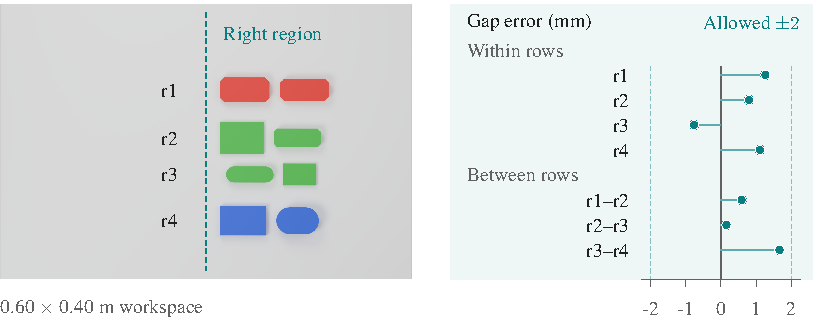
\includegraphics[width=\linewidth]{figures/layout_constraints.pdf}
\caption{\textbf{Region and spacing audit of the prediction in Figure~\ref{fig:motion}.} The overhead render preserves the scene geometry and poses, with a teal guide marking the right half of the workspace. The chart plots measured minus requested envelope gaps: 15\,mm within each of four rows and 30/15/30\,mm between the three row pairs. All seven errors lie within the shared $\pm2$\,mm tolerance.}
\label{fig:layout_constraints}
\end{figure}

\begin{table}[H]
\centering\small
\caption{Stored source and predicted poses and their differences, using the IDs in Figure~\ref{fig:motion}. Positions and distances are in millimeters, and angles are in degrees. Values are rounded to two decimal places for display; the audit archive retains full precision.}
\label{tab:motion_poses}
\setlength{\tabcolsep}{3pt}
\begin{tabular*}{\linewidth}{@{}r@{\extracolsep{\fill}}rrrrrrrr@{}}\toprule
& \multicolumn{3}{c}{Source pose} & \multicolumn{3}{c}{Predicted pose} & \multicolumn{2}{c}{Pose change} \\
\cmidrule(lr){2-4}\cmidrule(lr){5-7}\cmidrule(l){8-9}
\textbf{ID} & $x$ & $y$ & $\theta$ & $\hat x$ & $\hat y$ & $\hat\theta$ & $d$ & $\Delta\theta$ \\\midrule
1 & 369.01 & 206.60 & -3.92 & 355.05 & 205.63 & -0.05 & 13.99 & 3.86 \\
2 & 389.78 & 274.40 & -11.46 & 441.71 & 77.18 & -0.06 & 203.94 & 11.41 \\
3 & 495.33 & 279.53 & 41.90 & 359.72 & 280.29 & -0.05 & 135.60 & -41.96 \\
4 & 75.31 & 100.52 & 69.81 & 357.06 & 77.18 & -0.05 & 282.71 & -69.86 \\
5 & 248.50 & 175.74 & 84.43 & 444.44 & 148.91 & -0.07 & 197.76 & -84.51 \\
6 & 254.96 & 81.15 & 69.88 & 441.39 & 205.63 & -0.07 & 224.17 & -69.94 \\
7 & 164.85 & 186.67 & -17.60 & 367.66 & 148.91 & -0.07 & 206.30 & 17.53 \\
8 & 435.56 & 69.35 & -73.01 & 452.53 & 280.29 & -0.06 & 211.62 & 72.95 \\
\bottomrule
\end{tabular*}
\end{table}

\newpage
\paragraph{Coordinates and angle convention.}
The origin is the workspace's bottom-left corner, with $+x$ right and $+y$ up. Table~\ref{tab:motion_poses} converts stored meter/radian poses to millimeters/degrees without rewrapping individual angles. Euclidean displacement is $d_i=1000\|\hat p_i-p_i^{\mathrm{src}}\|_2$. For the undirected long axis, signed rotation is
\begin{equation}
\Delta\theta_i=\frac{180}{\pi}\left[\left(\hat\theta_i-\theta_i^{\mathrm{src}}+\frac\pi2\right)\bmod\pi-\frac\pi2\right].
\end{equation}
The resulting range is $[-90^\circ,90^\circ)$, with positive values indicating counterclockwise rotation. Object IDs link the saved poses to both Blender views. These endpoint differences do not specify path length or a collision-free manipulation sequence.

\paragraph{Geometry scope and precision.}
The four rows contain IDs $(3,8)$, $(1,6)$, $(7,5)$, and $(4,2)$. Their row-band gaps are 30.592, 15.159, and 31.668\,mm, within the requested 30/15/30\,mm bands. The right-half guide lies at $x=0.30$\,m. Nominal right-region limits are $0.32\leq x\leq0.58$\,m with a 0.1\,mm evaluator tolerance. Saved envelopes span $0.3210$--$0.4905$\,m. Gap errors use true rectangular envelopes at stored predicted poses, rather than center distances or rendered pixels. They describe this layout's geometry, not learned latent structure, holdout performance, or physical accuracy.

Source poses are archived in \code{audit/evidence/full8b\_choice.json}. The files \code{audit/layout\_constraints.json} and \code{audit/constraint\_correspondence.json} retain full-precision motion and spacing measurements, respectively. The former also records the rounded values in Table~\ref{tab:motion_poses}. Figure~\ref{fig:layout_constraints} uses the audited overhead Blender render with all object transforms and predictions preserved.

\end{document}
